
\centerline{\textbf{ \LARGE Pipeline }}

\begin{enumerate}
    \item Instruction Execution \\
        \begin{figure}[h]
            \centering   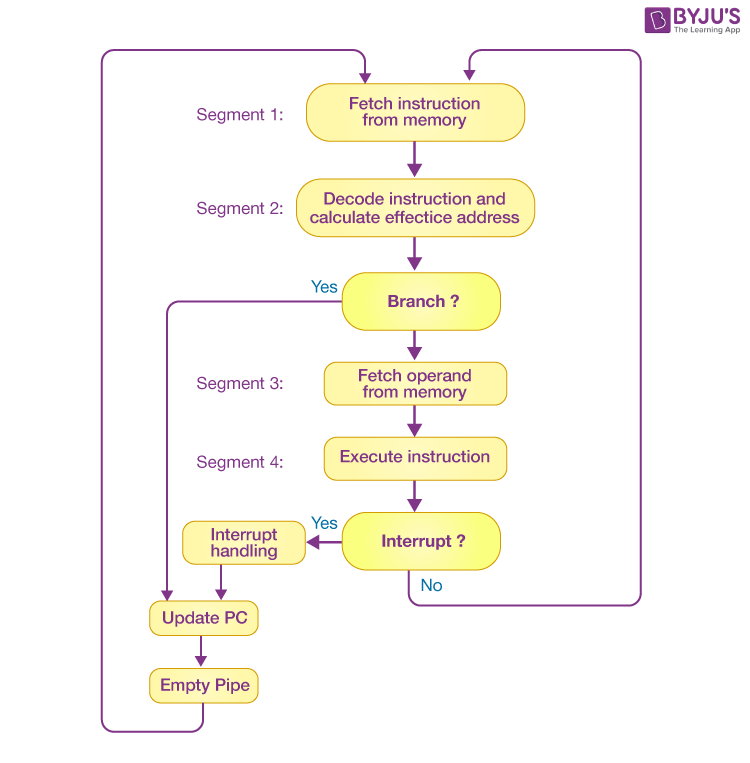
\includegraphics[scale=0.5]{./images/instruction-execution.png}
        \end{figure}

    \item Formulas\\
    \begin{myTableStyle} \begin{tabular}{ |m{5cm}|m{3cm}|m{5cm}| } \hline
        Stages                      &  k                & \\ \hline
        instructions                &  n                & \\ \hline
        Cycle Time                  &  \(T_c\)          &  Max(StageDelay) + Buffer Delay\\ \hline
        Total Cycles(Pipeline)      &  k + (n-1)        & \(Time = P_c * T_c\) \\ \hline
        Total Cycles(Non-Pipeline)  &  n*k              & \(Time = (NP)_c * T_c\) \\ \hline
        Speed-up                    &  n*k/(k + (n-1))  & = k, n \(\gg\) k. \\ \hline
    \end{tabular} \end{myTableStyle} \vspace{0.08in}

    \item Structural Hazards.
    \begin{enumerate}
        \item Hardware resource conflicts among the instructions in the pipelin.
        \item Memory, a GPR Register, or an ALU
        \item Fetch cycle and Execution cycle both may need ALU at the same time. Fetching involves calculating Effective Address.
        \item more than one instruction in the pipe requires access to the very same resource in the same clock cycle.
        \item Solution: Introduce bubble
        \item Solution: Separate memory for Instruction and Data.
        \item Solution: Use of register files. Allows access to one write register, and one read register.
    \end{enumerate}

    \item Data Hazards : RAW, WAR, WAW.
    \begin{enumerate}
        \item instruction is dependent on the results of a previous instruction.
        \item Solution: Re-order instruction by compiler.
        \item Solution: Introduce bubble or NOP instruction.
        \item Solution: Data forwarding sends data directly to the desired pipeline unit.
    \end{enumerate}

    \item Control Hazards
    \begin{enumerate}
        \item caused by branch instructions.
        \item Result of instruction determines the next instruction to be executed.
        \item Solution: Re-order instruction. The Compiler is used to implement this delayed branch.
        \item Solution: Introduce bubble(Stalling).
        \item Solution: Prediction.
        \item Solution: Dynamic Branch Prediction : Branch Table Buffer
        \item Branch penalty = total no of stalls.
        \item If the target address is present after the kth stage, then there will be (k – 1) stalls.
        \item Total number of stalls = Branch frequency * Branch Penalty
    \end{enumerate}
    \item zzz
    \item zzz
    \item  Control unit in a pipelined design
\end{enumerate}
